
%%%%%%%%%%%%%%%%%%%%%%% file typeinst.tex %%%%%%%%%%%%%%%%%%%%%%%%%
%
% This is the LaTeX source for the instructions to authors using
% the LaTeX document class 'llncs.cls' for contributions to
% the Lecture Notes in Computer Sciences series.
% http://www.springer.com/lncs       Springer Heidelberg 2006/05/04
%
% It may be used as a template for your own input - copy it
% to a new file with a new name and use it as the basis
% for your article.
%
% NB: the document class 'llncs' has its own and detailed documentation, see
% ftp://ftp.springer.de/data/pubftp/pub/tex/latex/llncs/latex2e/llncsdoc.pdf
%
%%%%%%%%%%%%%%%%%%%%%%%%%%%%%%%%%%%%%%%%%%%%%%%%%%%%%%%%%%%%%%%%%%%


\documentclass[runningheads,a4paper]{llncs}

\usepackage{amssymb,graphicx,multirow,algorithm,algorithmic,amsmath,makecell,color,url}
%\usepackage{natbib}
\usepackage[table,xcdraw]{xcolor}
\setcounter{tocdepth}{3}

\usepackage{subfigure}
\usepackage{empheq}

%\urldef{\mailsa}\path|{alfred.hofmann, ursula.barth, ingrid.haas, frank.holzwarth,|
%\urldef{\mailsb}\path|anna.kramer, leonie.kunz, christine.reiss, nicole.sator,|
%\urldef{\mailsc}\path|erika.siebert-cole, peter.strasser, lncs}@springer.com|
\newcommand{\keywords}[1]{\par\addvspace\baselineskip
\noindent\keywordname\enspace\ignorespaces#1}
\hyphenpenalty=5000
\tolerance=1000

\begin{document}


\mainmatter  % start of an individual contribution

% first the title is needed
\title{Semi-automatic Scribble Generation for Interactive Image Segmentation Evaluation}

% a short form should be given in case it is too long for the running head
\titlerunning{Scribble Generation for Interactive Image Segmentation Evaluation}

% the name(s) of the author(s) follow(s) next
%
% NB: Chinese authors should write their first names(s) in front of
% their surnames. This ensures that the names appear correctly in
% the running heads and the author index.
%
\author{Bingjie Jiang \and Tongwei Ren$^{*}$ \and Jia Bei}
%
\authorrunning{Bingjie Jiang, Tongwei Ren, Jia Bei}
% (feature abused for this document to repeat the title also on left hand pages)

% the affiliations are given next; don't give your e-mail address
% unless you accept that it will be published
\institute{$^{1}$ State Key Laboratory for Novel Software Technology, Nanjing University, China\\
$^{2}$ Software Institute, Nanjing University, China\\
bjie.jiang@gmail.com, rentw@nju.edu.cn, beijia@software.nju.edu.cn
}

\toctitle{Labelling Generation for Interactive Image Segmentation Evaluation}
\tocauthor{Bingjie Jiang, Tongwei Ren, Jia Bei}
\maketitle


\begin{abstract}
This paper proposes a semi-automatic labelling generation method for evaluating interactive segmentation algorithms. We analyze the differences between multiple user labels and the resulting variance in their segmentation results when applied to four state-of-the-art segmentation algorithms. We then figure out the underlying consistence between user labels on the level of defined superpixel group. We also prove the validity of points as input of interactive segmentation algorithms. Finally, we propose a semi-automatic labelling generation methodology and apply the auto-generated labels to four state-of-the-art algorithms. Our method provides an objective way to evaluate interactive segmentation methods and is aimed at reducing human labour needed in this field in the future.\textcolor{red}{(no more than 150 words)}


\keywords{Human interaction differences; Automatic labelling; Evaluation of interactive segmentation algorithms}
\end{abstract}


\section{Introduction}
% Interactive image segmentation is important
As the foundation of numerous multimedia applications, interactive image segmentation has been widely utilized in object recognition \cite{Bao13tip}, image retrieval \cite{Xu14icme}, scene analysis \cite{Li15tcsvt}, visual tracking \cite{Ren15mmsys}, social media mining \cite{Sang12tmm} and so on. It can effectively extract the desired objects from images with the assistance of manual labels, which is used to approximately outline the regions of objects. There have been several types of manual labels applied in the existing interactive image segmentation algorithms, including triple map, boundary box and scribble, in which scribble is commonly used for its simplicity and flexibility in labelling.

% requirement of interaction: suitable for different users, current evaluation approach and its drawbacks: does not consider multiple users or high human labor
For different users may provide various scribbles in labelling, an effective interactive image segmentation algorithm should be robust to scribbles, i.e., its performance should not be obviously influenced by the difference of scribbles. It requires to evaluate interactive image segmentation algorithms on the scribbles provided by numbers of users with sufficient variety. However, in the evaluations of the existing algorithms \textcolor{red}{***}, only the scribbles provided by one specific user is used to reduce human labor. Obviously, such evaluations are not sufficient for they contain high randomness in the performance of different segmentation algorithms in comparison. Moreover, if the scribbles are intentionally selected, the evaluations may have a bias to some algorithms, which may influence the fairness of the evaluations.

% The involved human interaction is required to be informative so that it could serve as effective inputs of certain image segmentation algorithms. Yet it should not involve too much human labor in consideration of real-life application. However, when it comes to the evaluation of these algorithms, the comparison can hardly be objective due to the limited label source and rather subjective human interferences. Usually, interactive image segmentation algorithms are tested upon user labels provided by a specific author or experiment. In this way, the situation of multiple users are neglected and the performance of segmentation result could heavily depend on certain batch of human labels, rendering the result not convincing enough when compared with other algorithms. In order to evaluate different algorithms in an objective and universal way, it is necessary to provide a large dataset of varied labels. But it should involve a great amount of time and human labour to set up such kind of database and many measures need to be taken to ensure the variety of this dataset. Under this guidance, we come up with the idea of generating semi-automatic labels using the ground truth of certain images. With the help of our automatically generated labels, the volume of the dataset can be greatly increased with little cost of time and labour. The work of establishing an image label dataset can therefore be largely reduced and the evaluation of segmentation algorithms can  be more objective.

% our work
To overcome the above problem, we propose a semi-automatic scribble generation approach for interactive image segmentation evaluation. The proposed approach still only requires one user to take participation in evaluation. Instead of just providing his/her scribbles, the user should generate the ground truths of segmentation results, which can be efficiently obtained after several interactions. Then, based on the ground truths, a number of scribbles with variety will be automatically generated to stimulate the labelling results provided by different users. Finally, interactive image segmentation algorithms can be comprehensively evaluated using the scribbles.

%This paper deals with the problem of evaluating interactive segmentation algorithms in an objective way. The contribution of this paper includes: (1)  Analysis of differences and consistence between different user labels in a quantitative way. By clustering pixels and further decomposing them into groups, we figured out both consistence and inconsistence of human labels and their influence on segmentation results.(2)A semi-automatic labelling generation method. Based on the consistence of user labels, we figured out the distribution of key component coverage rate and use it to select key features from the image for further labelling. (3) General evaluation of interactive segmentation methods. Our automatically generated labels are then applied to different methods and the performance of these methods are evaluated.

% paper organization
\textcolor{red}{The rest of the paper is organized as follows: In section.2, we introduced the related works. In section.3, we introduce the design of the dataset and experiment, and section.4 presents the idea of user interaction difference and the underlying consistence . In section.5 we describe the details of our label generation methodology, and section.6 analyzes the performance of four algorithms on the auto-generated labels. The paper concludes in section.7.}

\section{\textcolor{red}{Related Work}}

% existing interactive image segmentation methods
Many state-of-the-art algorithms in interactive image segmentation have been proposed, starting from Boycov et. al \cite{boykov2001interactive}, which utilizes max-flow/min-cut energy minimization to achieve foreground/background interactive segmentation. The Grabcut algorithm\cite{rother2004grabcut} further reduces the user interaction by allowing users to label a rectangle around the foreground object. In random walker \cite{grady2006random}, each pixel is assigned a maximal probability which a random walker could reach it starting from the corresponding labels. Bai and Sapiro come up with an interactive framework for soft segmentation and matting of natural images and videos in \cite{bai2007geodesic}. Gulshan\cite{gulshan2010geodesic} introduces a new shape constraint for interactive image segmentation by shifting from a single star to multiple stars and adopts Geodesic paths instead of Euclidean rays.

% existing evaluation methods
For segmentation algorithm evaluation, Martin et. al  \cite{martin2001database} presents an image database of a wide variety of natural scenes and its application to segmentation algorithm evaluation.  Unnikrishnan \cite{unnikrishnan2007toward} proposed the normalized probabilistic rand (NPR) index, which can be used to perform a quantitative comparison between image segmentation algorithms. Kevin McGuinness \cite{mcguinness2010comparative} developed a tool set for comparative evaluation of interactive segmentation algorithms. Moschidis and Jim Graham carried out systematic performance evaluation of three efficient image segmentation algorithms in \cite{moschidis2010systematic}, which focuses on their function as the computational part of an interactive segmentation system.

\section{Data Set}
% introduction of berkeley dataset
We construct our data set Berkeley Segmentation Dataset \cite{martin2001database} in size of 96 images. Each image contains at least one obvious object, which could be unambiguously explained to users. And these images are also representative of some major challenges of image segmentation, including fuzzy boundary, complex texture and complex lighting conditions. The ground truths of segmentation results are precisely hand-labelled for each image to avoid biases.

% our labelling (including how to collect the labels)
To analyze the rules for scribble generation, we invite five users to manually label the images with The K-Space Segmentation Tool Set \cite{mcguinness2008k}. All the users are the students with basic computer operating skills but limited knowledge about interactive image segmentation. Each user is given a clear guidance and enough time to familiarize themselves with the labelling software, and all the labelling operations are carried out by mouse.

%Then in real experiment, each participants are provided with 96 images and the corresponding ground-truth which tells exactly which object to extract. However, we hide the segmentation result from user so that they will not realize if they have provided a "good" mark or not. We also confined the time for labeling each image. In this way, we manage to (1)limit the effort of participants to draw scribbles in consideration of real-life application.
%(2)obtain the most natural response of users rather than inputs guided by segmentation result.

\section{Analysis of Scribble Variety}
%\begin{figure}[h!]
%\centering
%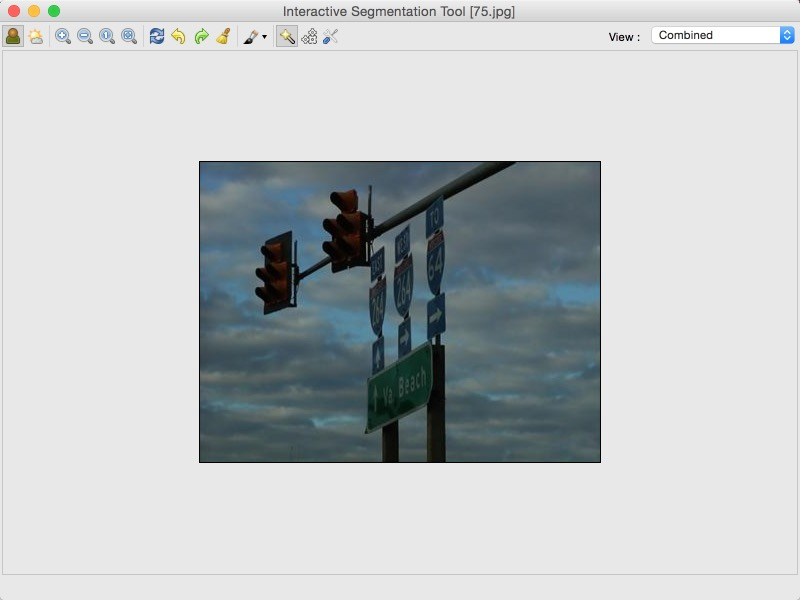
\includegraphics[width=0.5\columnwidth]{images/screenshot.png}
%\textbf{\caption{ The screenshot of k-space segmentation tool}}
%\label{fig:screenshot}
%\end{figure}

An instinctive observation is that different users cannot keep high consistency of scribble generation in labelling images. In order to validate the observation, we analyze the variety of scribbles labelled by different users. To facilitate the following description, we indicate the five users with $A$, $B$, $C$, $D$, and $E$. To the $k$th image, the scribbles labelled by user $n$ are represented as $s^{k}_{n}$, here $n\in \{A,B,C,D,E\}$. And the scribbles labelled by user $n$ on all the images are represented as $S_{n}$.

\subsection{Scribble difference}

We first analyze the difference of scribbles by pair-wise intersection rate. To the $k$th image, the intersection rate of the scribbles labelled by user $m$ and $n$ is calculated as $\phi^{k}_{m,n}=(s^{k}_{m}\cap s^{k}_{n})/(s^{k}_{m}\cup s^{k}_{n})$. And the average intersection rate of all the scribbles labelled by user $m$ and $n$ is calculated as $\bar{\phi}_{m,n}=\frac{1}{K}\sum^{K}_{k=1}{s^{k}_{m,n}}$, here $K=96$ is the number of images in our data set. Table \ref{tab:s-ir} shows the average interaction rates between the scribbles labelled by all the users on foreground and background, respectively. It is observed that the values of average intersection rates between the scribbles labelled by different users are quite low.


%In our person-oriented experiments, great differences among user labels were observed. It comes to us instinctively that different people tend to consider different parts of foreground and background object as salient. Under this guidance, we processed the 5 label files of the same image and calculated the pair-wise intersection rate. The result is shown in Table \ref{ta:intersection rate f} and \ref{ta:intersection rate b}. The pair-wise intersection rate is defined as follows: $$intersection\ of\ marked\ pixels/union\ of\ marked\ pixels$$ We make the following observations: (1)The value of intersection/union between every two people is quite small, which indicates that labels made by different people have little in common. Figure \ref{fig:example} shows an example of user labels which share no common pixels (2) People share less similarities in background labels than foreground. It is mainly because the foreground objects are confined to a certain area while the backgrounds are more extensive.


\begin{table}[!h]
\centering
\vspace{-0.2cm}
\caption{Pixel level average intersection rates of different scribbles on foreground and background.}
\begin{tabular}{c|c|c|c|c|c||c|c|c|c|c|c}
\hline
\multicolumn{6}{c||}{foreground} &\multicolumn{6}{c}{background}\\
\hline
& $S_{A}$ & $S_{B}$ & $S_{C}$ & $S_{D}$ & $S_{E}$ && $S_{A}$ & $S_{B}$ & $S_{C}$ & $S_{D}$ & $S_{E}$ \\
\hline
$S_{A}$ & -- & 2.4\% & 3.5\% & 2.0\%& 1.7\% &$S_{A}$ & -- & 0.9\% & 0.9\% & 0.1\%& 0.6\% \\
\hline
$S_{B}$ & 2.4\% & -- & 2.7\% & 2.2\%& 2.3\% &$S_{B}$ & 0.9\% & -- & 1.0\% & 0.2\%& 0.7\% \\
\hline
$S_{C}$ & 3.5\% & 2.7\% & -- & 2.1\%& 2.0\% &$S_{C}$ & 0.9\% & 1.0\% & -- & 0.2\%& 0.7\%\\
\hline
$S_{D}$ & 2.0\% & 2.2\% & 2.1\% & -- & 1.8\% &$S_{D}$ & 0.1\% & 0.2\% & 0.2\% & -- & 0.7\% \\
\hline
$S_{E}$ & 1.7\% & 2.3\% & 2.0\% & 1.8\%& -- &$S_{E}$ & 0.6\% & 0.7\% & 0.7\% & 0.7\% & -- \\
\hline
\end{tabular}
\label{tab:s-ir}
\end{table}


%\begin{table}[!tb]
% \centering
% \caption{intersection rate of foreground labels}
% \begin{tabular}{|c|c|c|c|c|c|}
% \hline
%  Label & label 1 & label 2 & label 3 & label 4& label 5 \\
% \hline
% label 1 & 100\% & 2.38\% & 3.52\% & 2.01\%& 1.66\% \\
% \hline
% label 2 & 2.38\% & 100\% & 2.71\% & 2.17\%& 2.25\% \\
% \hline
% label 3 & 3.52\% & 2.70\% & 100\% & 2.05\%& 2.01\%\\
% \hline
% label 4 & 2.01\% & 2.17\% & 2.05\% & 100\%& 1.84\% \\
% \hline
% label 5 & 1.66\% & 2.25\% & 2.01\% & 1.84\%& 100\% \\
% \hline
% \end{tabular}
% \captionsetup{justification=centerlast}
% \label{ta:intersection rate f}
% \end{table}

% \begin{table}[!tb]
% \centering
% \caption{intersection rate of background labels}
% \begin{tabular}{|c|c|c|c|c|c|}
% \hline
%  Label & label 1 & label 2 & label 3 & label 4& label 5 \\
% \hline
% label 1 & 100\% & 0.87\% & 0.86\% & 0.09\%& 0.63\% \\
% \hline
% label 2 & 0.87\% & 100\% & 0.97\% & 0.21\%& 0.73\% \\
% \hline
% label 3 & 0.86\% & 0.97\% & 100\% & 0.16\%& 0.68\%\\
% \hline
% label 4 & 0.09\% & 0.21\% & 0.16\% & 100\%& 0.67\% \\
% \hline
% label 5 & 0.63\% & 0.73\% & 0.68\% & 0.67\% & 100\% \\
% \hline
% \end{tabular}
% \captionsetup{justification=centerlast}
% \label{ta:intersection rate b}
% \end{table}


\begin{figure}[!tb]
\centering
\subfigure[source image] { \label{fig:a}
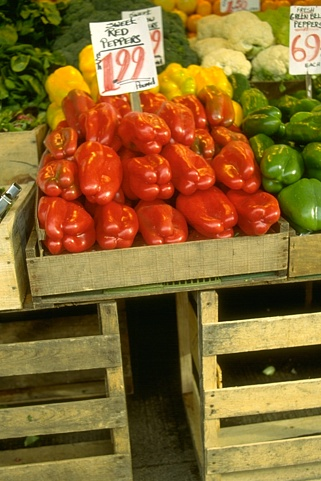
\includegraphics[width=0.15\columnwidth,height=1in]{images/25098-ori.jpg}
}
\subfigure[ground truth] { \label{fig:b}
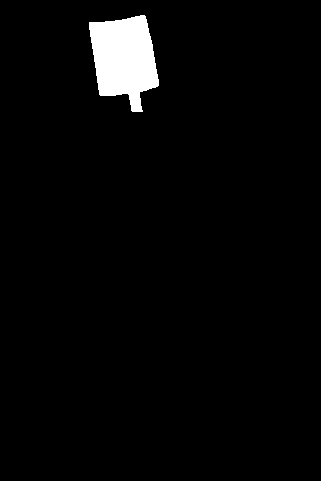
\includegraphics[width=0.15\columnwidth,height=1in]{images/25098-gt.png}
}
\subfigure[label1] { \label{fig:c}
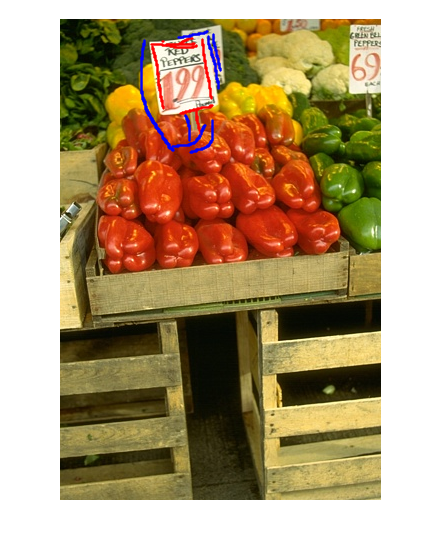
\includegraphics[width=0.15\columnwidth,height=1in]{images/25098-label-example-1.png}
}
\subfigure[label2] { \label{fig:d}
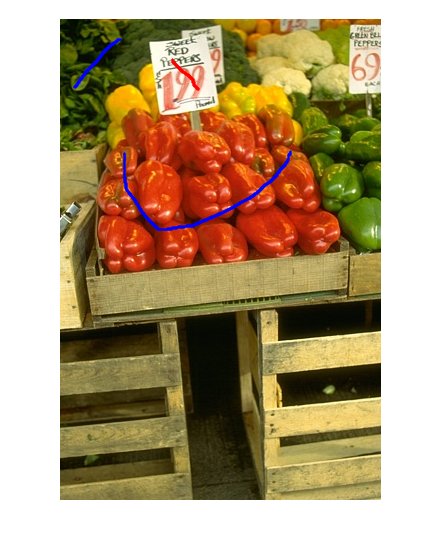
\includegraphics[width=0.15\columnwidth,height=1in]{images/25098-label-example-2.png}
}
\subfigure[auto label] { \label{fig:e}
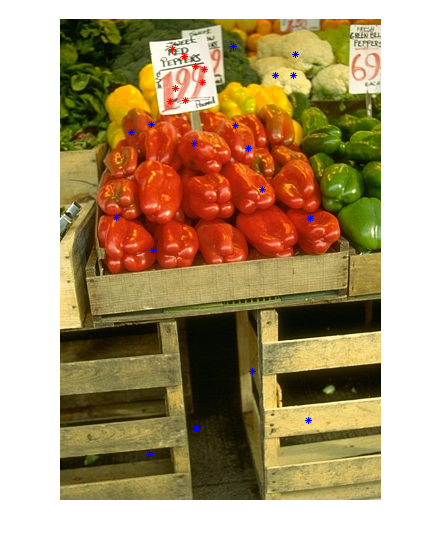
\includegraphics[width=0.15\columnwidth,height=1in]{images/25098-auto-label.png}
}
\subfigure[source image] { \label{fig:f}
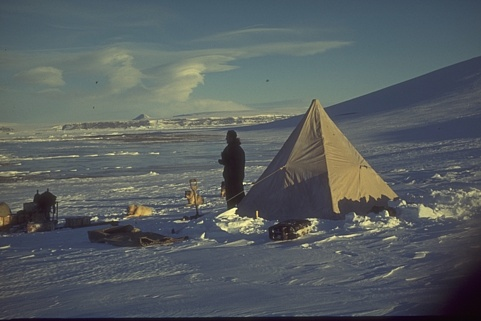
\includegraphics[width=0.15\columnwidth,height=1in]{images/188063-ori.jpg}
}
\subfigure[ground truth] { \label{fig:g}
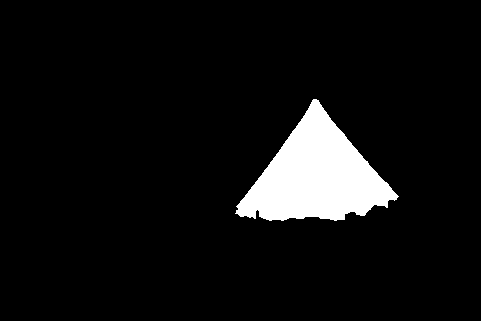
\includegraphics[width=0.15\columnwidth,height=1in]{images/188063-gt.png}
}
\subfigure[label1] { \label{fig:h}
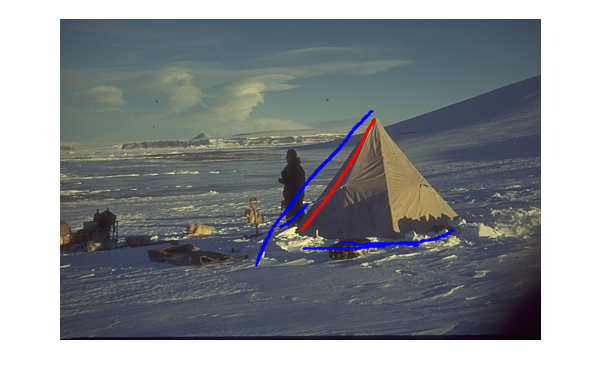
\includegraphics[width=0.15\columnwidth,height=1in]{images/188063-label-example-1.png}
}
\subfigure[label2] { \label{fig:i}
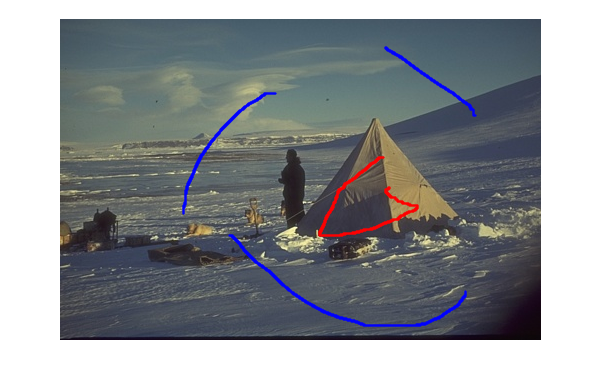
\includegraphics[width=0.15\columnwidth,height=1in]{images/188063-label-example-2.png}
}
\subfigure[auto label] { \label{fig:j}
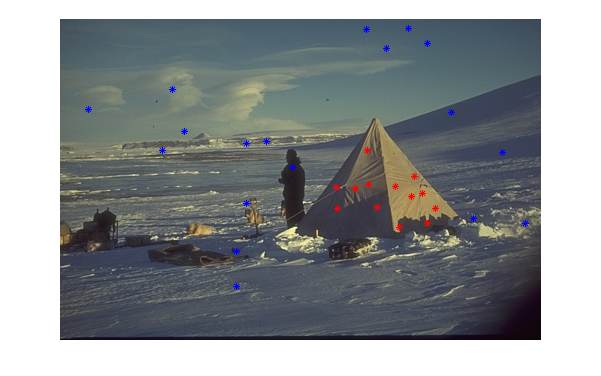
\includegraphics[width=0.15\columnwidth,height=1in]{images/188063-auto-label.png}
}

\caption{Examples of human labels and auto-generated labels. (a)(f) Source images. (b)(g) Ground truth of image(a)(f). (c)(d)(h)(i) Two pair of labels which share almost no common pixels. (e)(j) Examples of our auto-generated labels.}
\label{fig:example}
\end{figure}


\subsection{Influence to segmentation result}

We further evaluate the influence of different scribbles to segmentation results. We utilize the scribbles labelled by different users as the inputs of interactive image segmentation algorithms. In our experiments, four interactive image segmentation algorithms, including graph cut (GC) \cite{boykov2001interactive}, geodesic star convexity (GSC) \cite{gulshan2010geodesic}, random walker (RW) \cite{grady2006random}, and geodesic shortest path (GSP) \cite{bai2007geodesic}, which are provided by the implementation in \cite{gulshan2010geodesic}. Totally, $96\times 5\times 4$ segmentation results are generated by the four algorithms initialized with all the scribbles. To the five segmentation results generated by one algorithm on each original image, we calculate the percentages of pixels which occur as foreground in one, two, three, four or five segmentation results, respectively.

Fig. \ref{fig:segment} shows the boxplots of pixel co-occurrence percentages in different numbers of segmentation results for each segmentation algorithm. We can observe that the pixel co-occurrence percentages declines greatly when the number of segmentation results increases for all the algorithms. It means the segmentation results generated by the scribbles from different users are quite inconsistent. Moreover, to some segmentation algorithms which can generated relatively higher consistent results, such as GC and GSC, we can also find that their segmentation results contains high variability (larger lengthes of the boxes in Fig. \ref{fig:segment} (a) and (b)). Therefore, multiple scribbles with sufficient variety is required for comprehensively evaluating the performance of interactive segmentation algorithms.

%Based on the above result, we take a step further by examining the segmentation results of different labels.The implementation of four interactive segmentation algorithms in \cite{gulshan2010geodesic} was used. These algorithms are: Boykov Jolly Graph cut\cite{boykov2001interactive},  Boykov Jolly with Geodesic Star-Convexitycitep\cite{gulshan2010geodesic} , Bai and Sapiro Shortest Path\cite{bai2007geodesic} and Random Walker\cite{grady2006random}. 
%Based on the 96*5*4 segmentation results, we have found out that due to the variance between different labels, the segmentation results tend to be quite different, too.  We arrived here by calculating percentage of pixels which was segmented out as foreground simultaneously by 1 person, two people, three people ,four people and 5 people.
%The result is shown in Figure \ref{fig:segment}. We have observed that: (1) The intersection rate of segmented object declines greatly as the intersection scale expands, which means when there are multiple users, the segmentation results of a same image could be quite different. (2) While having a high intersection rate, segmentation results of BJ and GSC exhibits more variability than RW and SP, as indicated by the much larger length of box.

% (1) The effectiveness of different labels as input of interactive segmentation algorithms vary from person to person, as could be observed that the label made by participant 1 have a better performance than others in terms of mean, maximum and minimum, which means there exists kind of "professional lables" \cite{fu2008saliency} (2) On mean level, the result reaches at most 66.76\% made by participant 1. While the maximum ratio could be high as 99.05\%, the minimum ratio was also low as 1.06\%. This shows that when applied to segmentation algorithms, the variance of labels could further lead to even greater difference in segmentation results.


\begin{figure}[!h]
\centering
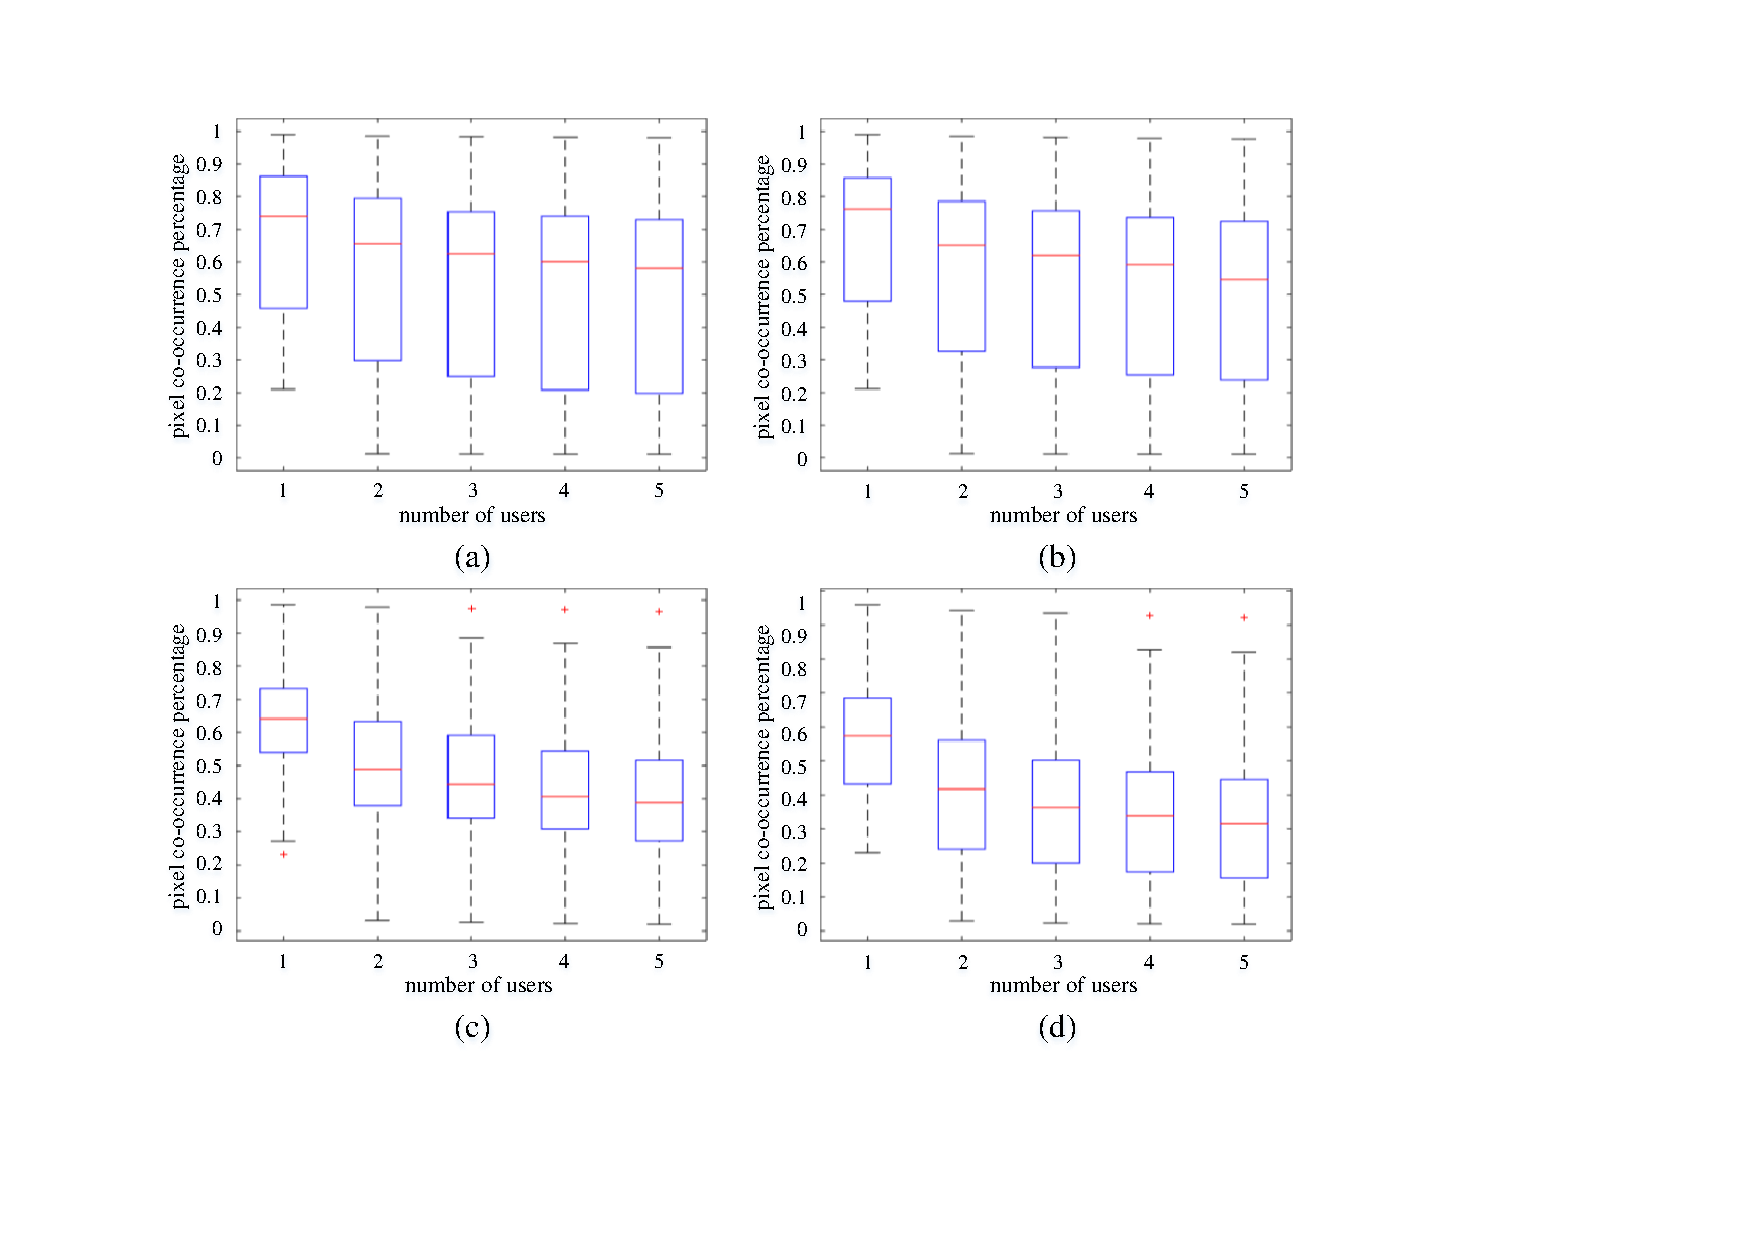
\includegraphics[width=0.9\textwidth]{fig_segment.pdf}
\caption{Percentages of pixel co-occurrence as foreground in different numbers of segmentation results. (a) GC. (b) GSC. (c) RW. (d) GSP.
%This figure shows the intersection of segmentation result of four algorithms on the five batches of labels. The five boxplot in each figure respectively shows the pixels which are segmented out simutaneously by one person, two people, three people, four people and five people.
}
\label{fig:segment}
\end{figure}

%\begin{figure}[!tb]
%\centering
%\subfigure[BJ] { \label{fig:a1}
%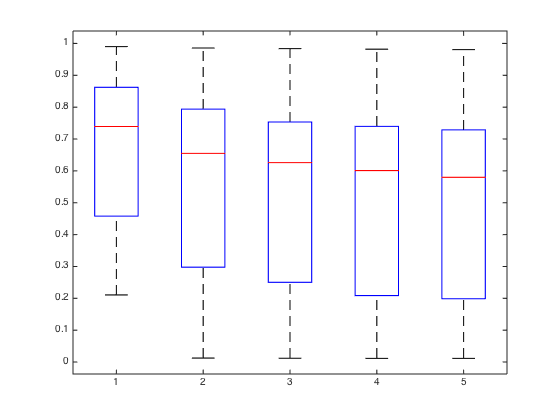
\includegraphics[width=0.4\columnwidth]{images/bj-seg-inter.png}
%}
%\subfigure[GSC] { \label{fig:b1}
%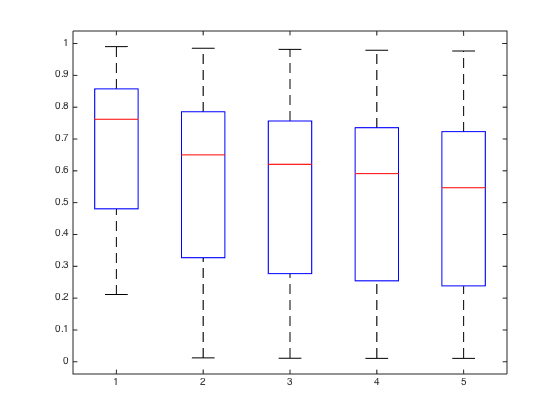
\includegraphics[width=0.4\columnwidth]{images/gsc-seg-inter.png}
%}
%\subfigure[RW] { \label{fig:c1}
%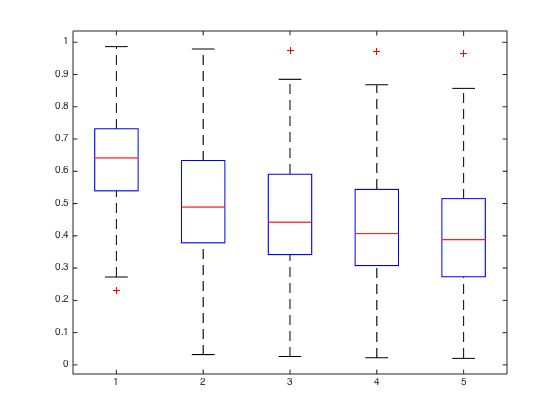
\includegraphics[width=0.4\columnwidth]{images/rw-seg-inter.png}
%}
%\subfigure[SP] { \label{fig:d1}
%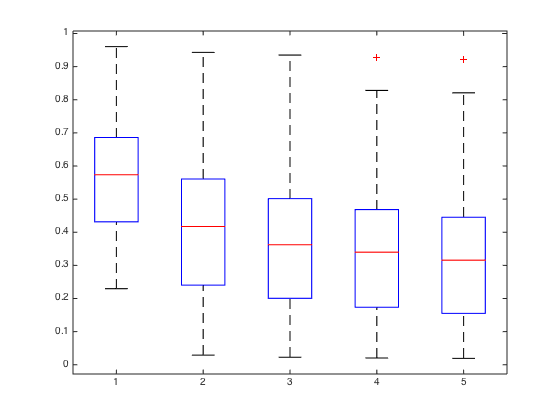
\includegraphics[width=0.4\columnwidth]{images/sp-seg-inter.png}
%}
%\caption{ This figure shows the intersection of segmentation result of four algorithms on the five batches of labels. The five boxplot in each figure respectively shows the pixels which are segmented out simutaneously by one person, two people, three people, four people and five people.}
%\label{fig:seg-inter}
%\end{figure}


\section{Semi-automatic Scribble Generation}

\subsection{Scribble consistency on superpixel and superpixel group levels}

For the scribbles labelled by different users have high inconsistence on pixel level, we analyze the scribbles on superpixel levels for expecting high consistency. we use the simple linear iterative clustering algorithm \cite{achanta2010slic}, which is implemented by VLFeat open source library \cite{vedaldi08vlfeat}, to cluster image pixels into compact and nearly uniform superpixels. To each superpixel, we consider it to be labelled by a scribble if one or more pixels in it are labelled by the scribble. Similar to pixel-level scribble consistency analysis, we analyze the scribble consistency on superpixel level by calculating the pair-wise intersection rates of the scribbles labelled by different users, which are calculated in a similar way to intersection rates of different scribbles on pixel level.

%To the $k$th image, the intersection rate of the scribbles labelled by user $m$ and $n$ on superpixel level is calculated as $\varphi^{k}_{m,n}=(sp^{k}_{m}\cap sp^{k}_{n})/(sp^{k}_{m}\cup sp^{k}_{n})$, here $sp^{k}_{m}$ and $sp^{k}_{n}$ denote the scribbles labelled by user $m$ and $n$ on the $k$th image. And the average intersection rate of all the scribbles labelled by user $m$ and $n$ on superpixel level is calculated as $\bar{\varphi}_{m,n}=\frac{1}{K}\sum^{K}_{k=1}{s^{k}_{m,n}}$, here $K=96$ is the number of images in our data set.

Table \ref{tab:sp-ir} shows the intersection rates of the scribbles labelled by different users on superpixel level. Here, $SP_{n}$ denotes all the scribbles labelled by user $n$ on superpixel level. Compared to pixel level analysis in Table \ref{tab:s-ir}, the scribbles have higher consistency on superpixel level than on pixel level, but the values of intersection rates are not high enough especially on background.

\begin{table}[!h]
\centering
\vspace{-0.2cm}
\caption{Superpixel level average intersection rates of different scribbles on foreground and background.}
\begin{tabular}{c|c|c|c|c|c||c|c|c|c|c|c}
\hline
\multicolumn{6}{c||}{foreground} &\multicolumn{6}{c}{background}\\
\hline
& $SP_{A}$ & $SP_{B}$ & $SP_{C}$ & $SP_{D}$ & $SP_{E}$ && $SP_{A}$ & $SP_{B}$ & $SP_{C}$ & $SP_{D}$ & $SP_{E}$ \\
\hline
$SP_{A}$ & -- & 49.3\% & 49.0\% & 38.9\% & 37.2\% & $SP_{A}$ & -- & 19.1\% & 17.8\% & 4.4\% & 11.9\% \\
\hline
$SP_{B}$ & 49.3\% & -- & 52.7\% & 43.5\% & 39.8\% & $SP_{B}$ & 19.1\% & -- & 21.2\% & 7.7\% & 15.2\% \\
\hline
$SP_{C}$ & 49.0\% & 52.7\% & -- & 41.6\% & 40.2\% & $SP_{C}$ & 17.8\% & 21.2\% & -- & 6.3\% & 16.1\% \\
\hline
$SP_{D}$ & 38.9\% & 43.5\% & 41.6\% & -- & 34.3\% & $SP_{D}$ & 4.4\% & 7.7\% & 6.3\% & -- & 16.1\% \\
\hline
$SP_{E}$ & 37.2\% & 39.8\% & 40.2\% & 34.3\% &--  & $SP_{E}$ & 11.9\% & 15.2\% & 16.1\% & 16.1\% & --  \\
\hline
\end{tabular}
\label{tab:sp-ir}
\end{table}

To further explore the consistency of different scribbles, we divide the superpixels into groups by quantifying them on RGB color space. We uniformly decompose R, G, B channels into eight parts and the whole RGB color space is decomposed into $8\times 8\times 8$ subspaces. All the superpixels whose average color belong to the same subspace are considered as a superpixel group. Similarly, if one or more pixels in a superpixel group are labelled by a scribble, we consider the superpixel group to be labelled by the scribble.

Table \ref{tab:sg-ir} shows the intersection rates of the scribbles labelled by different users on superpixel group level. Here, $SG_{n}$ denotes all the scribbles labelled by user $n$ on superpixel group level, and intersection rates of different scribbles are calculated in a similar way to intersection rates on pixel level and superpixel level. We can find that the consistency of scribbles on superpixel group level keeps increasing, and the values of intersection rates are rather high on both foreground and background.

\begin{table}[!h]
\centering
\vspace{-0.2cm}
\caption{Superpixel group level average intersection rates of different scribbles on foreground and background.}
\begin{tabular}{c|c|c|c|c|c||c|c|c|c|c|c}
\hline
\multicolumn{6}{c||}{foreground} &\multicolumn{6}{c}{background}\\
\hline
& $SG_{A}$ & $SG_{B}$ & $SG_{C}$ & $SG_{D}$ & $SG_{E}$ && $SG_{A}$ & $SG_{B}$ & $SG_{C}$ & $SG_{D}$ & $SG_{E}$ \\
\hline
$SG_{A}$ & -- & 77.7\% & 78.3\% & 73.2\% & 77.6\% & $SG_{A}$ & -- & 66.9\% & 67.1\% & 58.2\% & 68.1\% \\
\hline
$SG_{B}$ & 77.7\% & -- & 81.5\% & 78.4\% & 79.8\% & $SG_{B}$ & 66.9\% & -- & 68.6\%& 61.7\% & 70.2\% \\
\hline
$SG_{C}$ & 78.3\% & 81.5\% & -- & 78.4\% & 78.8\% & $SG_{C}$ & 67.1\% & 68.6\% & -- & 60.6\% & 70.5\% \\
\hline
$SG_{D}$ & 73.2\% & 78.4\% & 78.4\% & -- & 75.3\% & $SG_{D}$ & 58.2\% & 61.7\% & 60.6\% & -- & 66.1\% \\
\hline
$SG_{E}$ & 77.6\% & 79.8\% & 78.8\% & 75.3\%& --  & $SG_{E}$ & 68.1\% & 70.2\% & 70.5\% & 66.1\% & --  \\
\hline
\end{tabular}
\label{tab:sg-ir}
\end{table}

Based on the observation in Table \ref{tab:sp-ir} and \ref{tab:sg-ir}, we conclude that the scribbles labelled by different users are consistent on superpixel group level but keep some variety on superpixel level. The reason is that the key characteristics of foreground and background in each image are limited, and each key characteristic is represented by multiple superpixels especially on background. When a user labels an image, he/she usually tries to cover all the key characteristics of foreground and background to avoid further providing more interaction. Hence, most superpixel groups are labelled on both foreground and background. Nevertheless, the selection of superpixels to represent each key characteristic highly depends on personal habits. When a key characteristic is represented by multiple superpixels, the scribbles will appear obvious inconsistency.

% \subsection{Image representation for labelling quantitative analysis}
% In interactive image segmentation, users are expected labels some key features of the image foreground and background. The effectiveness of these labels is greatly related to their coverage of foreground and background key components. So we decide to simulate labels by simulating their coverage of key pixel groups. 
% In our method, we use the simple linear iterative clustering (SLIC)  method \cite{achanta2010slic} implemented by VLFeat open source library\cite{vedaldi08vlfeat}. The SLIC algorithm clusters pixels in the combined five-dimensional color and image plane space which brings compact, nearly uniform superpixels. 
% We then decompose all the superpixels into distinct groups according to the quantitative rgb feature of each superpixel. In this way, we could analyze user labels on both superpixel level and superpixel group level. On the level of superpixel, we are aimed at analyzing the amount of manual labour needed in providing certain labels; on the level of superpixel group, we could estimate the amount of information or key features provided by the labels.

\subsection{Content coverage by superpixel group}

To effectively stimulate the scribbles generated by different users, one important problem is how much image content should be covered by scribbles on superpixel group level, i.e., which percentage of superpixel groups should be labelled in scribble generation. To answer this question, we calculate the percentages of superpixel groups labelled as foreground and background by different users. Table \ref{tab:sg-coverage} shows the mean, variance and coefficient of variation (CV) of content coverage rate by superpixel groups on foreground and background, respectively. We can find that the content coverage rates of the scribbles labelled by different users only have small differences from similar mean values, and the content coverage rates of the scribbles labelled by the same user are stable from low values of variance and CV. Hence, in stimulating the scribbles labelled by one user, the content coverage rate can be randomly selected in a small range and it should be keep consistent in scribble generation.

%In order to generate automatic labels, we need to figure out the underlying consistence among labels made by different users. So we analyze the labels on both superpixel level and superpixel group level. Table \ref{ta: label coverage f}  and Table \ref{ta: label coverage b} show the coverage rate of superpixel groups in both foreground and background. We have observed that most of the defined superpixel groups are covered, which proves the representativeness of these groups. Also, inside single batch of labels which were made by the same user, the coverage rate is rather stable, as is indicated by low variance and coefficient of variance.

\begin{table}[!h]
\centering
\vspace{-0.2cm}
\caption{Content coverage rate by superpixel groups on foreground and background.}
\begin{tabular}{c|c|c|c|c|c||c|c|c|c|c|c}
\hline
\multicolumn{6}{c||}{foreground} &\multicolumn{6}{c}{background}\\
\hline
& $SG_{A}$ & $SG_{B}$ & $SG_{C}$ & $SG_{D}$ & $SG_{E}$ && $SG_{A}$ & $SG_{B}$ & $SG_{C}$ & $SG_{D}$ & $SG_{E}$ \\
\hline
mean & 74.9\% & 81.9\% & 83.6\%& 83.2\%& 76.5\% & mean & 64.9\% & 64.5\% & 65.4\%& 61.2\%& 74.1\% \\
\hline
variance & 0.03 & 0.03& 0.02& 0.02& 0.03 & variance & 0.03 & 0.02 & 0.02& 0.03& 0.02 \\
\hline
CV & 0.22 & 0.17 & 0.17& 0.18& 0.22 & CV & 0.27 & 0.21& 0.22& 0.31& 0.17 \\
\hline
\end{tabular}
\label{tab:sg-coverage}
\end{table}

%\begin{table}[!tb]
%\centering
%\caption{Superpixel group coverage in foreground.}
%\begin{tabular}{|c|c|c|c|c|c|c|}
%\hline
% & label 1 & label 2&label 3&label 4&label 5\\
%\hline
%Mean& 74.92\% & 81.91\% & 83.58\%& 83.18\%& 76.50\%\\
%\hline
%Variance& 0.03 & 0.03& 0.02& 0.02& 0.03 \\
%\hline
%CV & 0.22 & 0.17 & 0.17& 0.18& 0.22 \\
%\hline
%\end{tabular}
%\label{ta: label coverage f}
%\end{table}
%
%% CV: coefficient of variation
%\begin{table}[!tb]
%\centering
%\caption{Superpixel group coverage in background.}
%\begin{tabular}{|c|c|c|c|c|c|c|c|c|}
%\hline
% & label 1 & label 2&label 3&label 4&label 5 \\
%\hline
%Mean& 64.92\% & 64.46\% & 65.44\%& 61.15\%& 74.10\% \\
%\hline
%Variance& 0.03 & 0.02 & 0.02& 0.03& 0.02 \\
%\hline
%Coefficient of variance& 0.27 & 0.21& 0.22& 0.31& 0.17 \\
%\hline
%\end{tabular}
%\label{ta: label coverage b}
%\end{table}

\subsection{Effect of connection in scribble}

Another important problem in scribble generation is how to generate the smooth curves to represent the scribbles which should look natural and cover the prescribed percentage of superpixel groups. It is a very difficult and complex problem though it has been researched in computer graphics for years. To simplify the problem, we analyze the effective elements in scribble for interactive image segmentation.

To each scribble, we randomly select one superpixel from each superpixel group covered by the scribble and further randomly select one pixel from each superpixel. In this way, we obtain a pixel set as the representative of each scribble. Then, we generate the segmentation results using the scribbles and their corresponding pixel sets as the inputs respectively, and compare the segmentation results by the criteria of precision and recall.


%Instead of continuous user scribbles, our simulation is planned to generating points to represent key features in the image. So our first step was to validate the effectiveness of points in segmentation as compared to continuous lines. 
After figuring out the superpixel groups which were covered by certain user labels, we randomly select one superpixel from each group and then randomly select points from that superpixel. In this way, we formed a point set which contains points from groups covered by a certain human-made label. An example of our auto-generated label is shown in Figure \ref{fig:example}.  We then apply five sets of this kind of labels to the four segmentation algorithms. In terms of evaluation of segmentation accuracy, we use the commonly used precision and recall criteria.The precision and recall value of five batches of human-made labels and five batches of auto-generated labels applied to four algorithms are shown in Figure \ref{fig:pr-human-simu}. We have observed that our simulated label points achieves a very similar precision and recall level as human labels do. This strongly approves the validity of our assumption: discrete points which represent key features of the image could also act as effective labels.


%\begin{empheq}[box=\fbox]{align}
% \begin{split}
%  F_{gt} &= \text{foreground in ground truth}     \\
%  F_{s}  &= \text{foreground in segmentation}     \\
%   \text{recall}    &= \frac{F_{gt} \cap F_s}{F_{gt}}  \\
%   \text{precision} &= \frac{F_{gt} \cap F_s}{F_{s}}  \\
%   \end{split}
% \end{empheq}




\begin{figure}[!tb]
\centering
\subfigure[precision of BJ] { \label{fig:a1}
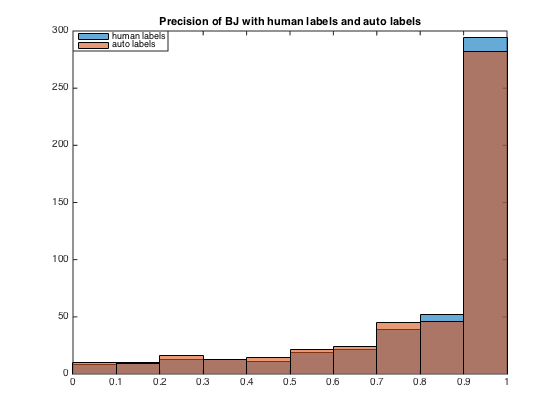
\includegraphics[width=0.4\columnwidth]{images/p_bj_human_auto.png}
}
\subfigure[precision of GSC] { \label{fig:a1}
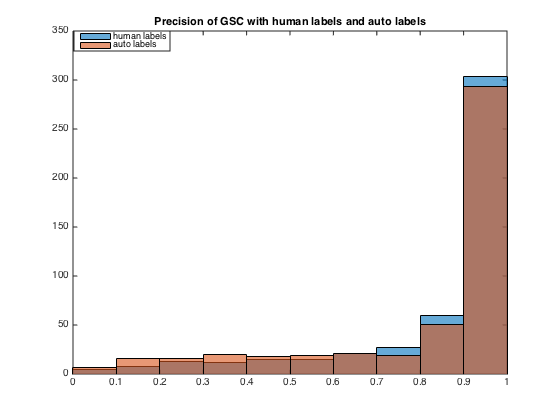
\includegraphics[width=0.4\columnwidth]{images/p_gsc_human_auto.png}
}
\subfigure[precision of RW] { \label{fig:a1}
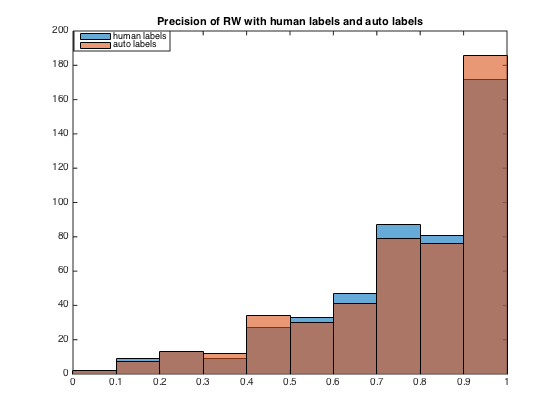
\includegraphics[width=0.4\columnwidth]{images/p_rw_human_auto.png}
}
\subfigure[precision of SP] { \label{fig:a1}
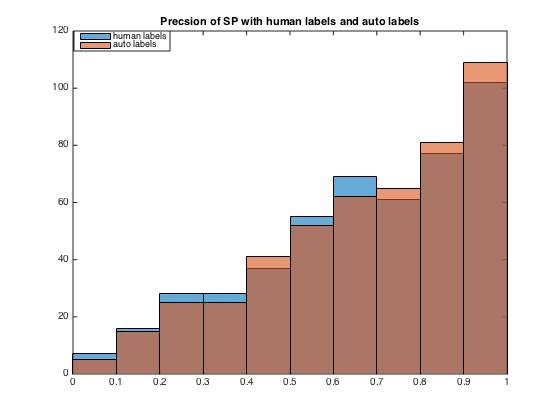
\includegraphics[width=0.4\columnwidth]{images/p_sp_human_auto.png}
}

\subfigure[recall of BJ] { \label{fig:a1}
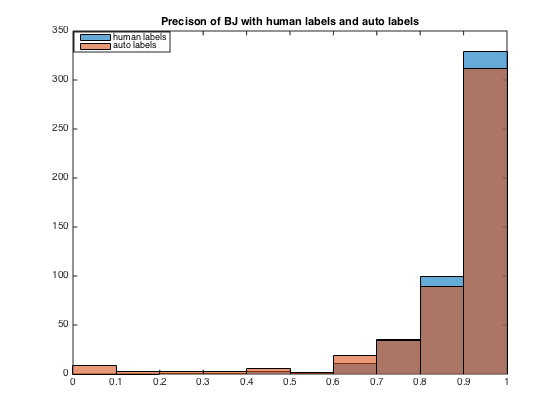
\includegraphics[width=0.4\columnwidth]{images/r_bj_human_auto.png}
}
\subfigure[recall of GSC] { \label{fig:a1}
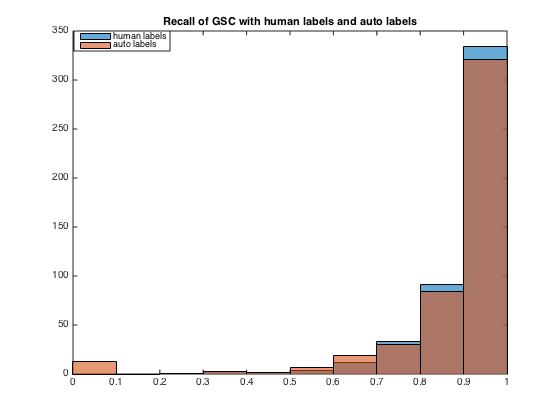
\includegraphics[width=0.4\columnwidth]{images/r_gsc_human_auto.png}
}
\subfigure[recall of RW] { \label{fig:a1}
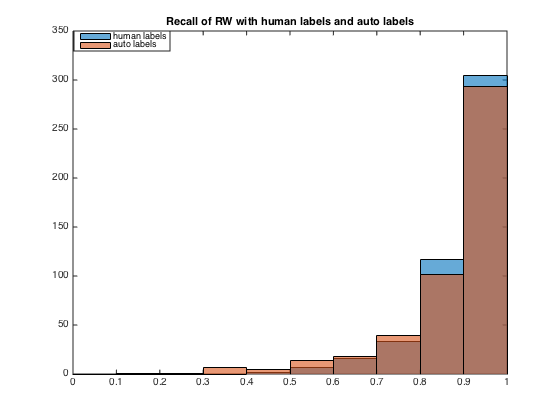
\includegraphics[width=0.4\columnwidth]{images/r_rw_human_auto.png}
}
\subfigure[recall of SP] { \label{fig:a1}
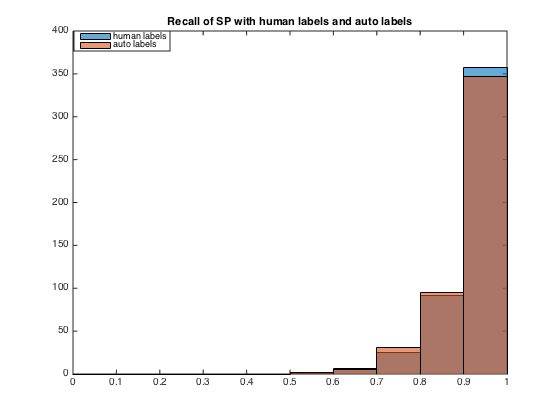
\includegraphics[width=0.4\columnwidth]{images/r_sp_human_auto.png}
}

\caption{ This figure shows the histogram of precision and recall value of segmentation result of four algorithms on both human labels and auto-generated labels.}
\label{fig:pr-human-simu}
\end{figure}

% Based on the rather stable level of group coverage, we calculate the group overlap rate between every two labels on the same image. Table \ref{ta:group overlap f} and Table \ref{ta:group overlap b}  shows the value in foreground and background. Value in position (i,j) denotes the percentage of groups in label i which were also covered in label j. We could note that the overlap rate between every two participants is rather high; We also examined the overlap percetage on superpixel level. Table \ref{ta: sp overlap f} and Table \ref{ta: sp overlap b} shows the result. It is obvious that different users share little common ground on superpixel level.



%\begin{table}[!tb]
%\centering
%\caption{Superpixel group overlap between labels in foregorund.}
%\begin{tabular}{|c|c|c|c|c|c|c|c|}
%\hline
% & label 1 & label 2&label 3&label 4&label 5&mean\\
%\hline
%label1& -- & 91.44\% & 92.86\%& 89.71\%& 88.64\%&90.66\%\\
%\hline
%label2& 83.86\% & -- & 90.75\%& 88.82\%& 85.93\%&87.34\%\\
%\hline
%label3& 83.40\% & 89.04\% & -- & 88.18\%& 84.62\%&86.31\% \\
%\hline
%label4& 80.75\% & 87.15\% & 88.15\%& -- & 82.44\%&84.62\% \\
%\hline
%label5& 82.53\% & 92.06\% & 92.10\%& 89.31\%& -- &90.00\% \\
%\hline
%\end{tabular}
%\label{ta:group overlap f}
%\end{table}
%
%\begin{table}[!tb]
%\caption{Superpixel group overlap between labels in backgorund.}
%\centering
%\begin{tabular}{|c|c|c|c|c|c|c|c|}
%\hline
% & label 1 & label 2&label 3&label 4&label 5&mean\\
%\hline
%label1& -- &80.19\% & 81.61\%& 72.23\%& 86.97\%&80.25\%\\
%\hline
%label2& 80.22\% & -- & 82.65\%& 74.86\%& 88.57\%&81.58\% \\
%\hline
%label3& 80.25\% & 81.42\% & -- & 74.09\%& 88.36\%&81.03\%\\
%\hline
%label4& 77.40\% & 80.30\% & 80.15\%& -- & 88.78\%&81.66\% \\
%\hline
%label5& 76.36\% & 77.76\% & 78.21\%& 73.21\%& -- &76.39\%\\
%\hline
%\end{tabular}
%\label{ta:group overlap b}
%\end{table}

% Based on analysis on superpixel and superpixel group level, we safely conclude that labels of different users are consistent on the defined superpixel group level but inconsistent on superpixel level. It is because that there are limited amount of key features of an object. But certain key features could always be represented by many different superpixels and users are usually sensitive to different representative superpixels.


%\begin{table}[!tb]
%\centering
%\caption{Superpixel overlap between labels in foreground.}
%\begin{tabular}{|c|c|c|c|c|c|c|}
%\hline
% & label 1 & label 2&label 3&label 4&label 5&mean\\
%\hline
%label1& -- & 3.70\% & 3.69	\%& 3.39\%& 3.35\%& 3.53\%\\
%\hline
%label2& 2.91\% & -- & 3.32\%& 3.14\%& 3.00\% & 3.09\%\\
%\hline
%label3& 2.78\% & 3.23\% & -- & 2.93\%& 2.90\%& 2.96\% \\
%\hline
%label4& 2.24\% & 2.63\% & 2.55\%& -- & 2.37\%& 2.45\%\\
%\hline
%label5& 2.25\% & 2.56\% & 2.58\%& 2.45\%& -- & 2.46\% \\
%\hline
%\end{tabular}
%\label{ta: sp overlap f}
%\end{table}
%
%
%\begin{table}[!tb]
%\centering
%\caption{Superpixel overlap between labels in background.}
%\begin{tabular}{|c|c|c|c|c|c|c|}
%\hline
% & label 1 & label 2&label 3&label 4&label 5&mean\\
%\hline
%label1& -- & 1.65\% & 1.59	\%& 0.49\%& 1.42\%& 1.29\%\\
%\hline
%label2& 1.70\% & -- & 5.33\%& 1.91\%& 1.81\%& 2.69\% \\
%\hline
%label3& 1.52\% & 1.75\% & --& 0.65\%& 1.77\%& 1.42\% \\
%\hline
%label4& 0.39\% & 0.64\% & 0.59\%& --& 1.56\%& 0.80\%\\
%\hline
%label5& 0.87\% & 1.08\% & 1.13\%& 1.18\%& --& 1.07\% \\
%\hline
%\end{tabular}
%\label{ta: sp overlap b}
%\end{table}


\subsection{Labelling generation}

In labelling generation, we test the normality of superpixel coverage distribution and superpixel-group coverage distribution.The Normal Q-Q plot of the four coverage rate is shown in Figure \ref{fig:histogram and qq plot}. As we can see from the plot, the data points of four plots are all close to the diagonal line.which indicates a normal distribution. We then fit the four distribution to normal distribution, and figure out the probability distribution function of both superpixel coverage percent and superpixel group coverage percent as $coverage \sim \mathcal{N} (m,\sigma^2)$, as is shown in Figure \ref{fig:histogram and qq plot} .Then our labelling generation process is carried out as following: For each image (1) We first generate two coverage percent of superpixel and superpixel group according to the calculated  distribution. (2) Randomly select superpixel groups according to the target percentage. (3) Select superpixels in each group for labelling according to the size of the group and the overall percentage.

\begin{figure}[!tb]
\centering
\subfigure[Normal Q-Q plot of superpixel group coverage rate in foreground] { \label{fig:a2}
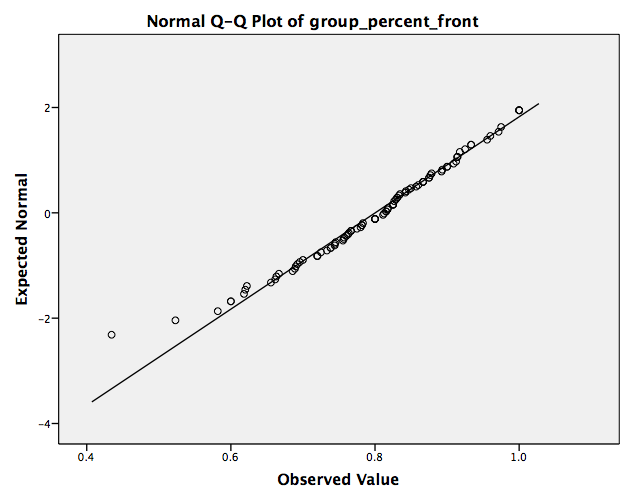
\includegraphics[width=0.4\columnwidth]{images/qq_group_f.png}
}
\subfigure[Normal Q-Q plot of superpixel group coverage rate in background] { \label{fig:b2}
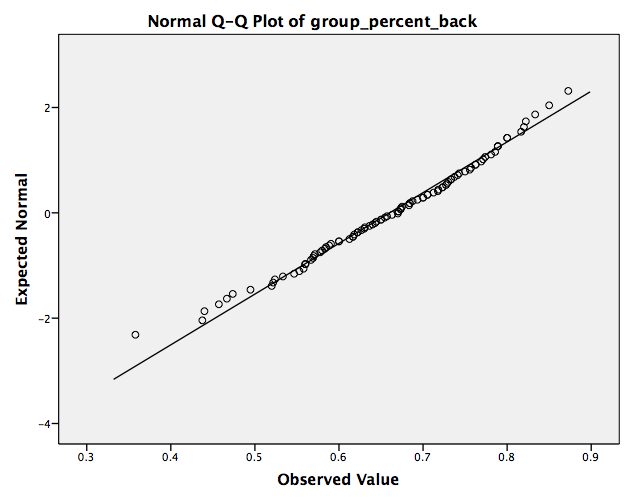
\includegraphics[width=0.4\columnwidth]{images/qq_group_b.png}
}
\subfigure[Normal Q-Q plot of superpixel coverage rate in foreground] { \label{fig:c}
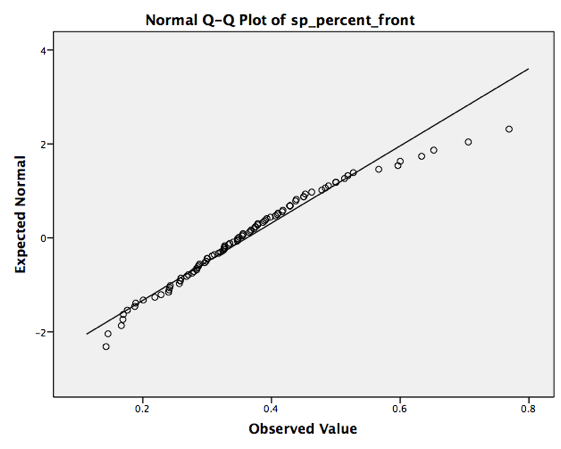
\includegraphics[width=0.4\columnwidth]{images/qq_sp_f.png}
}
\subfigure[Normal Q-Q plot of superpixel coverage rate in background] { \label{fig:c}
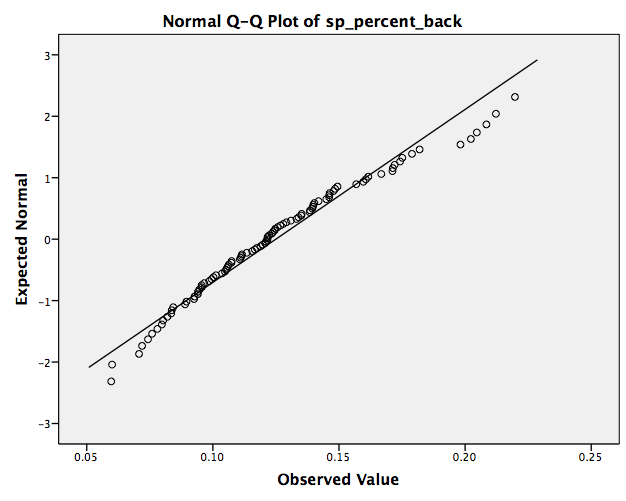
\includegraphics[width=0.4\columnwidth]{images/qq_sp_b.png}
}
%\caption{ Probability distribution of superpixel group/ superpixel  }
%\label{fig: qq plot}
%\end{figure}
%\begin{figure}[!tb]
%\centering
\subfigure[Distribution of superpixel group coverage rate in foreground ] { \label{fig:a2}
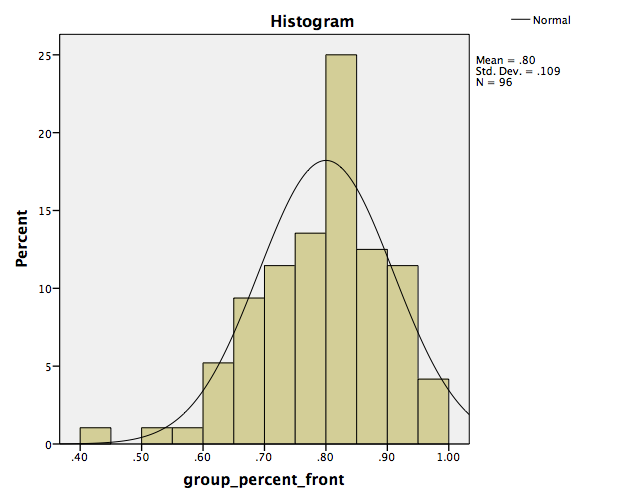
\includegraphics[width=0.4\columnwidth]{images/group_p_f.png}
}
\subfigure[Distribution of superpixel group coverage rate in background] { \label{fig:b2}
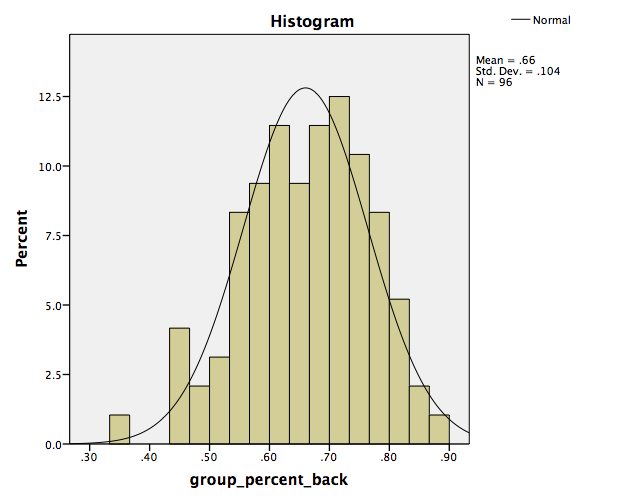
\includegraphics[width=0.4\columnwidth]{images/group_p_b.png}
}
\subfigure[Distribution of superpixel coverage rate in foreground] { \label{fig:c2}
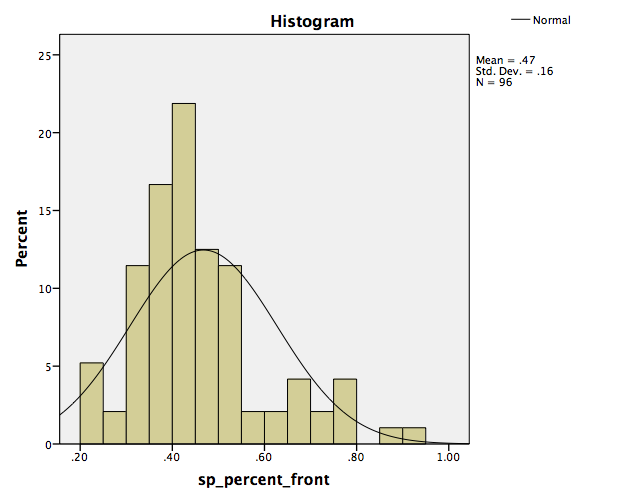
\includegraphics[width=0.4\columnwidth]{images/sp_p_f.png}
}
\subfigure[Distribution of superpixel coverage rate in background] { \label{fig:d2}
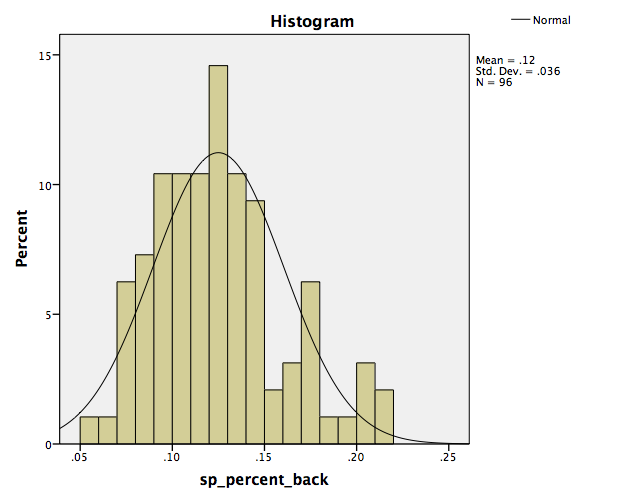
\includegraphics[width=0.4\columnwidth]{images/sp_p_b.png}
}
\caption{ This figure shows the probability distribution of superpixel group/ superpixel coverage in foreground and background }
\label{fig:histogram and qq plot}
\end{figure}


\section{Evaluation of Interactive Segmentation Algorithms}

We then test the four algorithms respectively with 96*5 auto-generated user labels and compare the result with the outcome of the previously made 96*5 human labels. We also provide labels generated in the following ways for comparison: (1) Randomly select a superpixel in each superpixel group for labelling(2) Randomly select certain percentage of superpixels among all superpixels without grouping them. In this way, we have four sets of labels in total. The result evaluation is shown in Figure \ref{fig:pr boxplot}. The first four figures show the precision values and the following four show the recall value. We make the following observations: (1) The performance of four algorithms remains similar under our auto-generated labels (the second column) compared with human-made labels, which confirms the stability of our simulation methods. It is thus promising that our auto-generated labels could serve as effective inputs of segmentation algorithms.(2) The third set of labels (the third column) are generated by covering all superpixel groups, thus providing more information than normal human labels could do.Sp it has much higher precision value than human labels do.(3) The fourth set of labels(the fourth column) is generated randomly on all superpixels. It shows the lowest precision level as it is formed by discrete superpixels, which can not provide enough information as superpixel groups could do.  (4) GSC \cite{gulshan2010geodesic} remains the best system on the whole dataset with high accuracy and stable performance. While RW \cite {grady2006random} and BJ \cite{boykov2001interactive}are expected to have similar performance, RW presents more robustness on both sets of labels. The SP\cite{bai2007geodesic} algorithm still achieves the poorest performance, mainly due to its lack of sensitivity to label locations.

\begin{figure}[!tb]
\centering
\subfigure[Precision value of BJ with human-made and auto-generate labels] { \label{fig:a3}
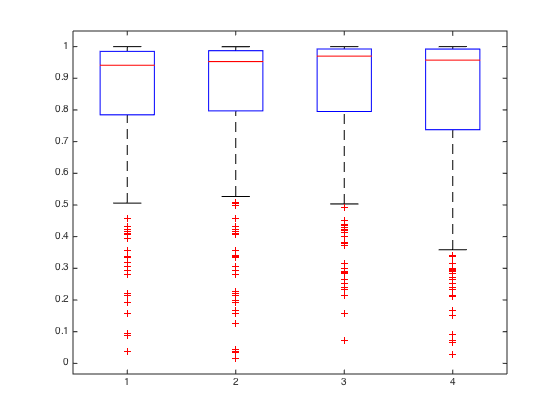
\includegraphics[width=0.4\columnwidth]{images/bj-eva-p.png}
}
\subfigure[Recall value of BJ with human-made and auto-generate labels] { \label{fig:b3}
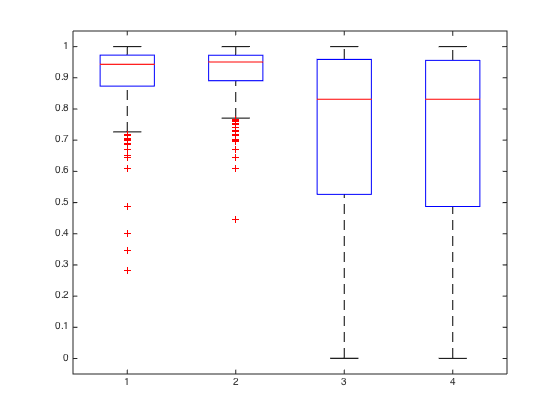
\includegraphics[width=0.4\columnwidth]{images/bj-eva-r.png}
}
\subfigure[Precision value of GSC with human-made and auto-generate labels] { \label{fig:c3}
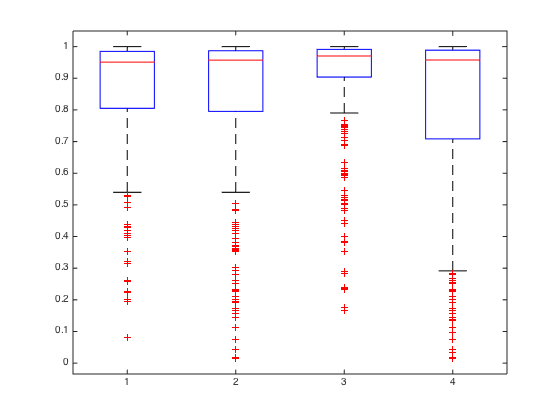
\includegraphics[width=0.4\columnwidth]{images/gsc-eva-p.png}
}
\subfigure[Recall value of GSC with human-made and auto-generate labels] { \label{fig:d3}
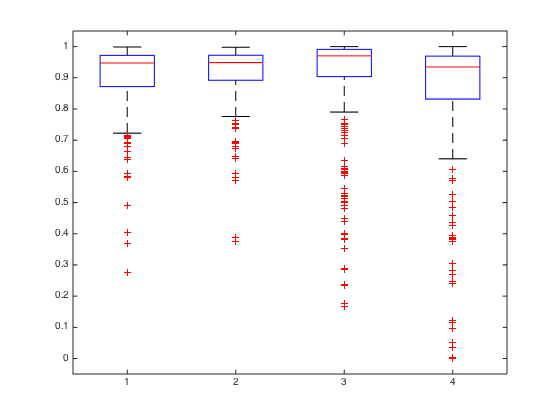
\includegraphics[width=0.4\columnwidth]{images/gsc-eva-r.png}
}
\subfigure[Precision value of RW with human-made and auto-generate labels] { \label{fig:e3}
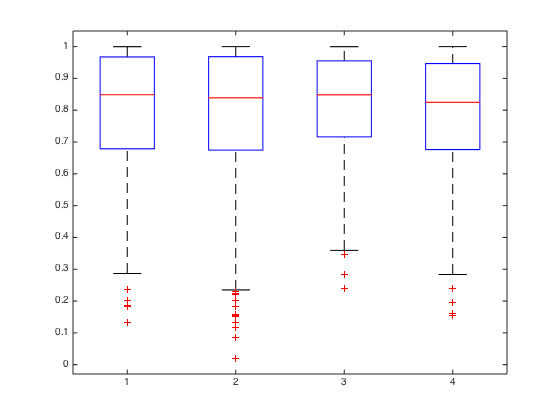
\includegraphics[width=0.4\columnwidth]{images/rw-eva-p.png}
}
\subfigure[Recall value of RW with human-made and auto-generate labels] { \label{fig:f3}
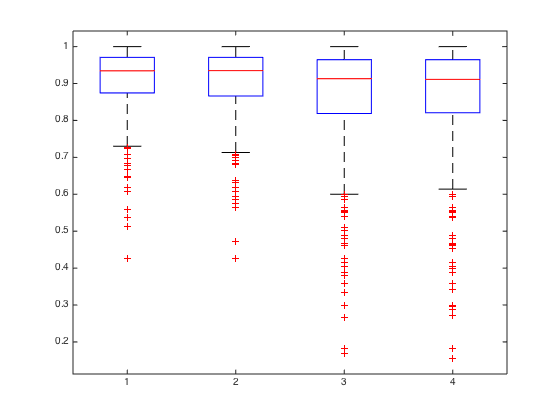
\includegraphics[width=0.4\columnwidth]{images/rw-eva-r.png}
}
\subfigure[Precision value of SP with human-made and auto-generate labels] { \label{fig:g3}
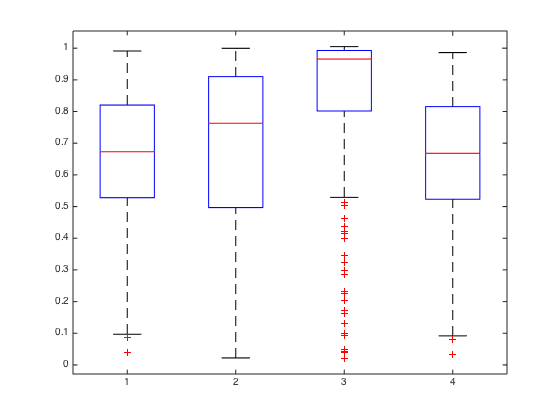
\includegraphics[width=0.4\columnwidth]{images/sp-eva-p.png}
}
\subfigure[Recall value of SP with human-made and auto-generate labels] { \label{fig:h3}
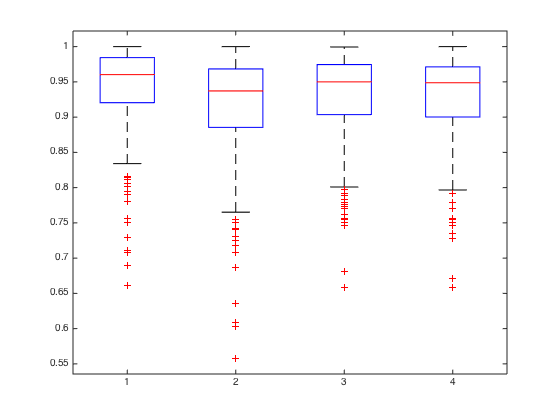
\includegraphics[width=0.4\columnwidth]{images/sp-eva-r.png}
}
\caption{This figure shows the precision/recall value of four algorithms with human-made and our auto-generated labels }
\label{fig:pr boxplot}
\end{figure}


\section{Conclusion}

In this paper, we propose a semi-automatic labelling generation method for evaluating interactive segmentation algorithms. We analyze the differences between multiple user labels and the corresponding segmentation results. Then we figure out the underlying consistence between user labels on the defined superpixel group level. After validating the effectiveness of point-level simulation, a labelling simulation methodology is proposed to simulate user labels. Finally, four state-of-art algorithms are tested and evaluated by the auto-generated labels.

\subsubsection*{Acknowledgments.} This work is supported by the National Science Foundation of China (61321491, 61202320), Research Project of Excellent State Key Laboratory (61223003), National Undergraduate Innovation Project (G1410284075) and Collaborative Innovation Center of Novel Software Technology and Industrialization.

%\bibliographystyle{plain}
%\bibliography{references}
\begin{thebibliography}{4}

\bibitem{Bao13tip} Bing-Kun Bao, Guangcan Liu, Richang Hong, Shuicheng Yan, and Changsheng Xu. General subspace learning with corrupted training data via graph embedding. IEEE Transactions on Image Processing. 22(11):4380--4393 (2013)

\bibitem{Xu14icme} Xiangyang Xu, Wenjing Geng, Ran Ju, Yang Yang, Tongwei Ren, Gangshan Wu. OBSIR: Object-based stereo image retrieval. IEEE International Conference on Multimedia and Expo. 1-6 (2014)

\bibitem{Li15tcsvt} Teng Li, Huan Chang, Meng Wang, Bingbing Ni, Richang Hong, and Shuicheng Yan. Crowded scene analysis: A survey. IEEE Transactions on Circuits and Systems for Video Technology. 25(3), 367--386 (2015)

\bibitem{Ren15mmsys} Tongwei Ren, Zhongyan Qiu, Yan Liu, Tong Yu, and Jia Bei. Soft-assigned bag of features for object tracking. Multimedia Systems. 21(2):189-205 (2015)

\bibitem{Sang12tmm} Jitao Sang, Changsheng Xu, Jing Liu. User-Aware image tag refinement via ternary semantic analysis. IEEE Transactions on Multimedia. 14(3-2):883--895 (2012)

\bibitem{boykov2001interactive} Yuri Y Boykov, and  Marie-Pierre Jolly. Interactive graph cuts for optimal boundary \& region segmentation of objects in N-D images. IEEE International Conference on Computer Vision. 105--112 (2001)

\bibitem{gulshan2010geodesic} Varun Gulshan, Carsten Rother, Antonio Criminisi, Andrew Blake, and Andrew Zisserman. Geodesic star convexity for interactive image segmentation. IEEE Conference on Computer Vision and Pattern Recognition. 3129--3136 (2010)
    
\bibitem{bai2007geodesic} Xue Bai and Guillermo Sapiro. A geodesic framework for fast interactive image and video segmentation and matting. IEEE International Conference on Computer Vision. 1--8 (2007)

\bibitem{grady2006random} Leo Grady. Random walks for image segmentation. IEEE Transactions on Pattern Analysis and Machine Intelligence. 28(11):1768-1783 (2006)




\bibitem{rother2004grabcut} Carsten Rother, Vladimir Kolmogorov, and Andrew Blake. Grabcut: Interactive foreground extraction using iterated graph cuts. ACM Transactions on Graphics. 23(3):309-314 (2004)

\bibitem{martin2001database} David Martin, Charless Fowlkes, Doron Tal, and Jitendra Malik. A database of human segmented natural images and its application to evaluating segmentation algorithms and measuring ecological statistics. IEEE International Conference on Computer Vision. 416--423 (2001)

\bibitem{mcguinness2010comparative} Kevin McGuinness and Noel E Oconnor. A comparative evaluation of interactive segmentation algorithms. Pattern Recognition. 43(2):434--444 (2010)

\bibitem{mcguinness2008k} Kevin McGuinness and Noel E OConnor. The k-space segmentation tool set. 2008.

\bibitem{fu2008saliency} Yu Fu, Jian Cheng, Zhenglong Li, and Hanqing Lu. Saliency cuts: An automatic approach to object segmentation. International Conference on Pattern Recognition. 1--4 (2008)

\bibitem{achanta2010slic} Radhakrishna Achanta, Appu Shaji, Kevin Smith, Aurelien Lucchi, Pascal Fua, and Sabine Susstrunk. Slic superpixels. Technical report (2010)

\bibitem{vedaldi08vlfeat} A. Vedaldi and B. Fulkerson. VLFeat: An open and portable library of computer vision algorithms. http://www.vlfeat.org/, 2008.

\bibitem{unnikrishnan2007toward} Ranjith Unnikrishnan, Caroline Pantofaru, and Martial Hebert. Toward objective evaluation of image segmentation algorithms. IEEE Transactions on Pattern Analysis and Machine Intelligence. 29(6):929-944 (2007)

\bibitem{moschidis2010systematic}Emmanouil Moschidis and Jim Graham. A systematic performance evaluation of interactive image segmentation methods based on simulated user interaction. IEEE International Symposium on Biomedical Imaging: From Nano to Macro, 928--931 (2010)

\end{thebibliography}

\end{document}
